\documentclass[Main]{subfiles}
\begin{document}

\chapter{Java Remote Method Invocation}
This chapter will cover the fundamentals in the distributed object-based system Java Remote Method Invocation (RMI) and how a leader of the distributed collaboration is elected.

\section{JAVA RMI}
Java Remote Method Invocation (RMI) is a middleware that supports Java-to-Java only. RMI gives a client on one Java Virtual Machine (JVM) access to objects that runs on another JMV which allows the client to invoke methods on the object - called the Remote Object. Thus providing remote communication between programs written in Java \cite{RMI-slides}. A JVM is a program that provides a run-time environment where applications written in Java binary code (called bytecode) can be executed. The JVM contains a set of instructions which is used when interpreting a Java bytecode enable the processor to execute a compiled Java program. The JVM will subsequently handle the actual execution of the program by interpreting each of its instructions, enabling automatic exception handling \cite[p. 422-423]{Tanenbaum}, \cite{wiki-jvm}.\\The remote object is a distributed object whose state always resides on one single JVM but whose interface can be made available to processes on another JVM \cite[p. 461]{Tanenbaum}.

\begin{figure}[H]
\centering
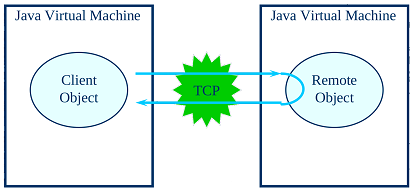
\includegraphics[scale=0.8]{Figurer/JVM.png}
\caption{System-overview of a Java RMI containing two JVM's \cite{RMI-slides}}
\label{Figure-jvm}
\end{figure}

The methods in the remote object can be accessed and invoked through an interface; the stub, which make the object appear as if it was a local object on the client's side. The interface is implemented as a proxy; a local representation of or placeholder for the remote object, which offers exactly the same interface as the remote object (the skeleton). The interface offers a declaration of the methods which can be invoked \cite[p. 461]{Tanenbaum}, \cite{RMI-slides}. During the communication between the two JVM's the complex data-structures which represents the object need to be transferred from one JVM to another. In order to facilitate this the object or its structures need to be serialized\footnote{The technique of serialization is typically called \textit{marshalling an object} in other programming languages than Java}; the data is translated into a format that can be transmitted across a network connection. The opposite operation; extracting a data-structure from a series of bytes is called deserialization \cite[p. 462]{Tanenbaum}, \cite{wiki-serialization}.

\subsection{The architecture and communication}
The architecture of the Java RMI is based on the principle that the definition of 'behavior' of an object and the implementation of that behavior is separate concepts. The Java RMI shown in Figure \ref{Figure-jvm} contains the elements introduced in the section above. A orderly and more detailed description of the communication and the three main layers; Stub and Skeleton Layer, Remote Reference Layer and Transport Layer follows:
\begin{itemize}

\item On the rightmost Java Virtual machine resides the \textbf{Server} which create and registers the remote objects interface; the skeleton

\item The \textbf{skeleton} is the server-side implementation of the remote object. It makes the method-calls to the actual object and accepting the return value before transmitting it to the stub. The skeleton takes care of the deserialization of the arguments send by the client (will be explained later) and the serialization of the objects and data-structures before the data is being transmitted to the client through a network.

\item On the leftmost Java Virtual machine resides the \textbf{Client}. The client invokes stub-methods and through these calls the client can use the facilities of the services provided by the application on the server.

\item The \textbf{stub} class is the proxy of the skeleton. It initiate a call to the remote object by calling the remote reference layer with serialized arguments. Thus it communicates with the skeleton and handles the deserialization when binary data is received through the network. Afterwards the stub informs the Remote Reference Layer that the call is complete.

\item The \textbf{Remote Reference Layer} interprets and manage the references made from client to the remote server object. It sets up the connection to the remote address. It is a middleware that manages the client-server connection via TCP/IP and transmits serialized data to the transport layer. This middleware is providing a transparent communication-way thus the developer is being provided a client-server communication when using this layer.

\item The \textbf{Java RMI registry} is a simplified name service offering a reference (the stub) to a remote object.
\begin{figure}[H]
\centering
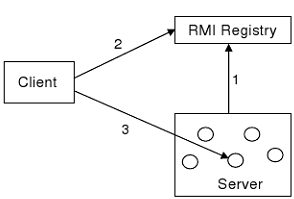
\includegraphics[scale=0.8]{Figurer/RMI-registry.png}
\caption{The use of the RMI Registry \cite{RMI-slides}}
\end{figure}
The registry is used to locate the remote object a Client need to use as it provides a name to a remote object's skeleton. Ones a remote object is registered on a server (1), clients can look up the objects by names (2) and obtain a remote object reference which is used to communicate with the wanted server and its remote object (3). Thus the registry provides the stub and the reference to the remote object \cite{Getting-started}.

\item The \textbf{Transport Layer} handles how the data is transported via the TCP/IP connection through a network. It is responsible for accepting calls on incoming connections, setting up the connection between JVM's and dispatch to the remote reference layer. It contains the following features:
\begin{itemize}
\item \textbf{Endpoint} used to denote the addresses to the client and the server; the address space or a JVM
\item \textbf{Channel} is responsible for managing the connection between the client and the server
\item \textbf{Connection} is used to transfer the data
\item \textbf{Transport}. Within a transport between a server and a client only one channel exist.
\end{itemize}

\setlength\parindent{300pt}\cite{RMI-slides}

\end{itemize}

MIA: Se evt. http://www.sce.carleton.ca/netmanage/simulator/rmi/RMIExplanation.htm og forklar RRL og Transport-layer bedre.

\section{Leader election}



\end{document}  